\chapter{Sample Chapter}

For all of those that know \LaTeX: please don't hurt me after what you see here. I'm just making a quick and dirty template. It's by no means perfect nor correct \LaTeX but at least it works.

\section{Section}
\subsection{Subsection}
\subsubsection{Subsubsection}
\paragraph{Paragraph}
Content :-D

\section*{Unnumbered section}
\section[short section title]{Long section title in text}

\section{Lists}
\begin{itemize}
  \item This
  \item Is
  \item A
  \item Simple
  \item List
\end{itemize}

\paragraph{Numbered list}

\begin{enumerate}
  \item This
  \item Is
  \item A
  \item Simple
  \item Numbered
  \item List
\end{enumerate}

Want to make some multiline text?\\What about \\ that

Empty line works as well. (makes new paragraph)

\section{Some math}
\label{section-math}
It has a lot of math abilities, some basic would be:

The Pytaghorean theorem \(x^2 + y^2 = z^2\)

or centered and in separate line \[ x^2 + y^2 = z^2 \]

You can also put equations like that: $E=mc^2$

How about greek letters?$\alpha \beta \gamma \delta \epsilon$

\section{Tables}
Tables? You got it (It can get scarry at this point, sort of similar to HTML tables)

\begin{center}
  \begin{tabular}{ c | l r }
   centered & left aligned & right aligned \\ \hline
   a2 & b1 & c2 \\  
   a3 & b3 & c3    
  \end{tabular}
  \end{center}
  
  Keep in mind that that's very basic example. Then you also have stuff like multipage tables, advanced tables etc.

\newpage
\section{images}
You can also add images. There are two main ways you might want to do that:

Cute cat:

\begin{center}
  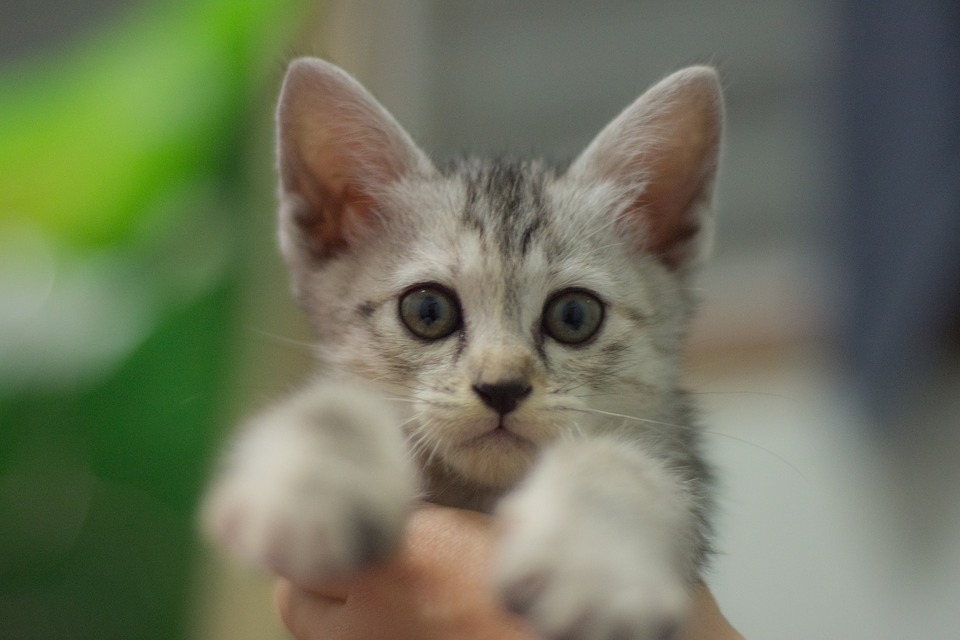
\includegraphics[width=0.8\textwidth]{cat1}
\end{center}

Or you can use figures like on \autoref{fig-picture} (just keep in mind that figures will be placed not where you want but where \LaTeX\space thinks its best to put it (you can obviously override this either by giving subtle hints like in the example or completely))

\begin{figure}[h]
  \centering
  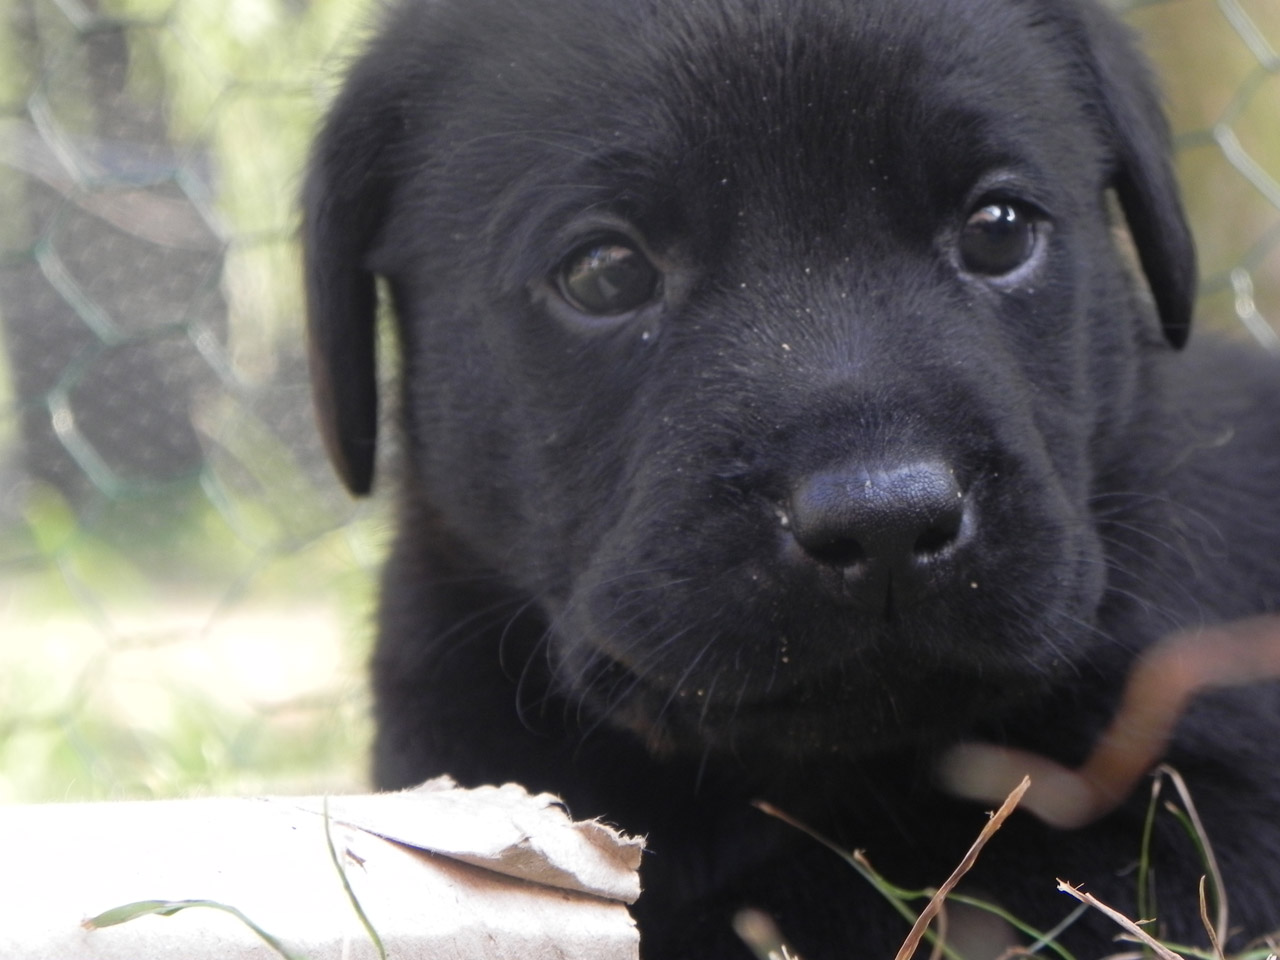
\includegraphics[width=0.8\textwidth]{puppy}
  
  \caption{\label{fig-picture}Just kidding, dogs are much cuter}
\end{figure}

\section{Hyperlinks}

You can put hyperlinsk to a lot of stuff but probably most useful are:
\begin{itemize}
  \item link to other place in the document (to the label) like to section \ref{section-math}. You can also use autoref to have automatic location type like with \autoref{fig-picture}. You can also just make it to a given page \pageref{fig-picture}.
  \item Link to the URL, like for example to Overleaf here: \url{https://www.overleaf.com/learn/latex/Main_Page} where they have a way better \LaTeX tutorial than this thing.
\end{itemize}